\documentclass[font=default]{mpltx}

% 以下至 \begin{document} 都仅是本文件为了方便额外定义的命令, 写报告时不需要.
\hypersetup{colorlinks=true}% 超链接带颜色
\usepackage{xcolor}
\newcommand{\note}[1]{{\color{gray}#1}}
\NewDocumentCommand{\pkg}{s o m}{%
    \IfBooleanF{#1}{%
        \IfNoValueTF{#2}%
            {\href{https://www.ctan.org/pkg/#3}}%
            {\href{https://www.ctan.org/pkg/#2}}%
    }%
    {\textsf{#3}}%
}
\newcommand*\cs[1]{\texttt{\textbackslash #1}}
\newcommand*\env[1]{\textit{\texttt{#1}}}
\newcommand*\code[1]{\texttt{#1}}
\newcommand*\file[1]{\textbf{\texttt{#1}}}
\makeatletter
\newcommand\releasedate{%
    \href{https://github.com/CastleStar14654/PKUMpLtX/releases/tag/\mpltx@fileversion}%
        {\mpltx@filedate, \mpltx@fileversion}}
\makeatother
% 以上是本文件为了方便额外定义的命令, 写报告时不需要.
\linespread{1.5}
\begin{document}

\title{塞曼效应} % 切合报告内容, 简短明确, 可以不同于讲义
\author{MaskedName} % 这里 \emailphone 一定要紧跟在 \author 后方
\emailphone{MyMail@stu.pku.edu.cn}{Tel}
% 如果改用 \email 则仅需要邮箱参数
\affiliation{北京大学物理学院\quad 学号: StudentID}
% % 可以使用 \zhdate 自动生成中文日期, 如
% \date{\zhdate{2020/12/1}}
% % 也可使用 babel 的 \localedate, 如
% \date{\localedate{2020}{12}{1}}
% % 两者均会输出 `2020 年 12 月 1 日'
% 下面的 \date 的参数是为了自动输出正确版本号, 正式报告请替换为上面的两种 \date 之一
\date{\zhdate{2023/9/20}}
\begin{abstract}
塞曼效应是指原子在外磁场中发光谱线发生分裂的现象,是研究原子结构的十分重要的途径之一.本实验通过气压扫描式法布里-珀罗标准具(F-P标准具)测量了汞灯546.1 nm谱线在无磁场,0.8 T以及1 T磁场下的塞曼谱线,并对谱线进行了一定程度的分析.本实验从光谱的分析中得到了各子谱线和546.1 nm线的波数差以及相对强度,并与理论计算结果比较,简要分析了误差的来源.本实验还通过光谱计算了电子的荷质比,并与标准值进行比较,发现两者十分接近,证实了理论的正确性.
\end{abstract}
\keywords{波数差,子谱线, F-P标准具}

\maketitle

\section{引言}
1896年,荷兰物理学家塞曼(Pieter Zeeman)发现了将钠光源放在足够强的外磁场中,一条谱线会分裂成几条偏振化的谱线,后来人们称此现象为``塞曼效应''(为区分没有磁场作用的光谱线,我们称磁场作用分裂后的光谱线为子谱线).随后洛伦兹在理论上解释了谱线分裂成3条的原因,并得到谱线的裂距等于一个洛伦兹单位($\widetilde{L}=eB/4\pi mc$).但是进一步的研究发现,很多原子的光谱在磁场中的分裂情况非常复杂,需要用量子理论才能解释,这种现象称为``反常塞曼效应''.

塞曼效应是继``法拉第效应''和``克尔效应''之后,第三个用来说明磁场和电场对光产生影响的例证.从塞曼效应的结果中人们可以得到有关能级的数据,即由分裂后子谱线的个数可以知道能级的$J$值,从子谱线裂距的大小可以知道$g$因子.这个现象的发现是对光的电磁理论的有力支持,证实了磁矩和空间取向量子化,使人们对物质光谱、原子、分子有了更深入的了解.因此,塞曼效应被誉为继X射线之后物理学最重要的发现之一.

本实验中,我们使用气压扫描式法布里-珀罗标准具(简称F-P标准具,一种分辨本领较高的分光仪器)观察并研究汞(Hg)放电灯的546.1 nm光谱线在外磁场作用下的塞曼分裂结果,并且可以观察到谱线的超精细结构.通过对光谱的分析,我们可以得到子谱线的波数差和相对强度,最终我们可以求出荷质比.将实验测量结果与理论相比照,可以让我们更加深入的了解塞曼效应,将原子物理和量子力学的理论知识同实验联系起来.

\section{理论\cite{Book}}
\subsection{原子的总磁矩和总角动量的关系}
严格来讲,原子的总磁矩由电子磁矩和核磁矩两部分组成,但是由于后者比前者小三个数量级,所以这里我们暂时只考虑电子磁矩的影响.电子磁矩由两部分构成:电子绕原子核作轨道运动而产生的轨道磁矩,与电子自旋产生的自旋磁矩.根据量子力学的结果,电子的轨道角动量$\bm{P_L}$和轨道磁矩$\bm{\mu_L}$以及自旋角动量$\bm{P_S}$和自旋磁矩$\bm{\mu_S}$有如下关系$$\bm{\mu_L}=-\frac{e}{2m}\bm{P_L},\quad \bm{P_L}^2=L(L+1)\frac{h^2}{4\pi^2},\quad \bm{\mu_S}=-\frac{e}{m}\bm{P_S},\quad \bm{P_S}^2=S(S+1)\frac{h^2}{4\pi^2}.$$其中$e,m$分别表示电子电荷和电子质量;$L,S$分别表示轨道角动量量子数和自旋角动量量子数.记轨道角动量和自旋角动量合成的总角动量为$\bm{P_J}$,合成的总磁矩为$\bm{\mu_J}$如 \autoref{fig1} 所示.

按照 \autoref{fig1} 进行矢量运算可以得到$\bm{P_J}$和$\bm{\mu_J}$之间的关系为
\begin{equation}\label{eq1}
    \langle \bm{\mu_J}\rangle =-g\frac{e}{2m}\langle\bm{P_J}\rangle.
\end{equation}
其中
\begin{equation}\label{eq_g}
  g=1+\frac{J+(J+1)-L(L+1)+S(S+1)}{2J(J+1)},
\end{equation}
为朗德(Lande)$g$因子,它表征了单电子的总磁矩和总角动量之间的关系.若是具有两个或者两个以上的电子,可以证明磁矩$\bm{\mu_J}$与原子的总角动量$\bm{P_J}$的表达式与 \autoref{eq1} 相同,但是$g$因子随着耦合类型不同有不同的计算方法.
\begin{figure}
    \centering
    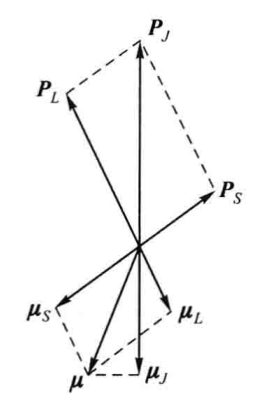
\includegraphics[width=4cm]{fig/01.png}
    \caption{\centering 角动量和磁矩矢量图}
    \label{fig1}
\end{figure}
\subsection{外磁场对原子能级的影响}
原子的总磁矩在外磁场中会受到力矩的作用,并得到附加的能量
\begin{equation}\label{eq2}
    \Delta E=-\bm{\mu_J}\cdot\bm{B}=g\frac{e}{2m}P_{J_z}B,
\end{equation}
其中$P_{J_z}$是$z$方向上的角动量.根据量子理论,$z$方向的角动量也是分立的,其量子化条件为
\begin{equation}
    P_{J_z}=M\frac{h}{2\pi},\quad M=J,J-1,\cdots,-J,\label{eq3}
\end{equation}
共有$2J+1$个$M$值,将 \autoref{eq3} 代入 \autoref{eq2} 可以得到
\begin{equation}\label{eq4}
    \Delta E=Mg\frac{eh}{4\pi m}B.
\end{equation}这样,无外磁场时的一个能级,在外磁场的作用下分裂成$2J+1$个子能级,每个能级附加的能量由 \autoref{eq4} 决定,它正比于外磁场$B$和朗德$g$因子.
\subsection{塞曼能级跃迁的选择定则}
对应于能级$E_2$和$E_1$之间的跃迁,光谱线的频率$\nu$满足下式:$$\nu=\frac{1}{h}(E_2-E_1).$$在磁场中能级分裂后,附加的能量分别为$\Delta E_2$和$\Delta E_1$,新的谱线频率为$$\nu'=\frac{1}{h}(E_2+\Delta E_2)-\frac{1}{h}(E_1+\Delta E_1),$$分裂谱线的频率差为$$\Delta\nu=\nu'-\nu=\frac{1}{h}(\Delta E_2-\Delta E_1)=(M_2g_2-M_1g_1)\frac{eB}{4\pi m}.$$分裂谱线的波数差为
\begin{equation}\label{eq5}
  \Delta\widetilde{\nu}=(M_2g_2-M_1g_1)\frac{eB}{4\pi mc}=(M_2g_2-M_1g_1)\widetilde{L},
\end{equation}其中
\begin{equation}\label{eq6}\widetilde{L}=\frac{eB}{4\pi mc}=0.467B,
\end{equation}称为洛伦兹单位.

选择定则告诉我们$\Delta M=0,\pm 1$.当$\Delta M=0$时,垂直于磁场观察时产生线偏振光,线偏振光的振动方向平行于磁场,称为$\pi$线.当$\Delta M=\pm 1$时,垂直于磁场观察时,产生线偏振光,线偏振光的振动方向垂直于磁场,称为$\sigma$线(注意在平行于磁场观察时,会产生圆偏振光,转动方向依赖于$\Delta M$的正负号.但是本实验不进行平行于磁场的观察).根据辐射过程中,原子和发出的光子作为整体的角动量守恒这一原理,可以解释偏振光现象.
\subsection{分裂谱线的强度}
本实验用到的汞灯546.1 nm发光谱线是由双电子${\rm 6s7s^3S_1\to 6s6p^3P_2}$的跃迁产生的.
垂直于磁场观察,根据偶极辐射的自发射概率公式,以及考虑到偏振态,可以得到在垂直于磁场观察时各线相对强度的理论公式:

对于$J\to J+1$跃迁:
\begin{equation}\label{eq8}
  M_J\to M_J\pm 1,\quad I_\sigma=\frac{1}{4}(J\pm M_J+1)(J\pm M_J+2);\quad M_J\to M_J,\quad I_\pi=(J+1)^2-M_J^2.
\end{equation}
上述结果只适用于弱场下的塞曼分裂(弱场指外磁场相对于原子自身的自旋轨道耦合作用比较弱,不会破坏原子内部的耦合运动).

根据 \autoref{eq5}, \autoref{eq6} 和 \autoref{eq8} 我们可以计算出各子谱线相对于无磁场时谱线的位置以及子谱线的相对强度.最后结果由 \autoref{fig_spectrum} 所示,由此我们可以得到理论上塞曼效应的结果.
\begin{figure}
  \centering
  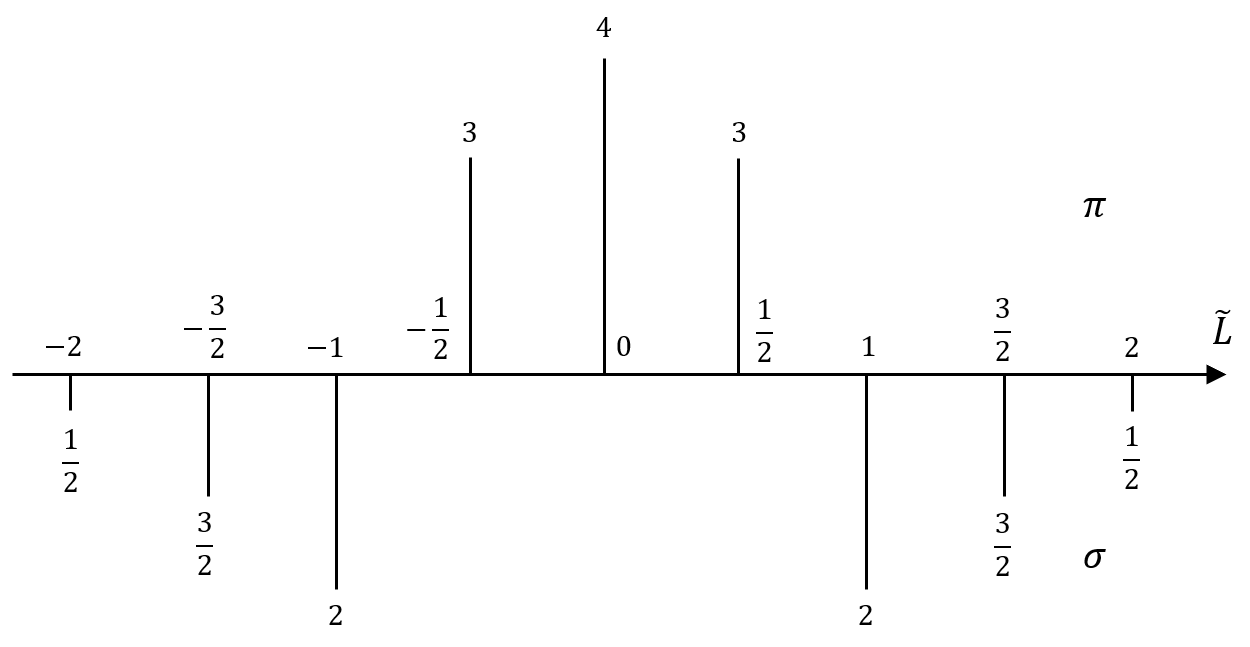
\includegraphics[width=0.75\linewidth]{fig/spectrum.png}
  \caption{汞546.1 nm谱线的塞曼分裂示意图.横轴表示各条子谱线相对于无磁场时谱线的位置,单位为洛伦兹单位$\widetilde{L}$.横线上的竖线表示$\pi$成分,横线下的竖线表示$\sigma$成分,线段的长度表示谱线的相对强度,用 \autoref{eq8} 计算得到.}
  \label{fig_spectrum}
\end{figure}
\subsection{超精细结构}
用大型光栅光谱仪和法布里-珀罗标准具等高分辨率仪器拍摄元素的光谱时,会看到更细致的结构,称为超精细结构.超精细结构主要是由核自旋以及核电四极矩引起的.在本实验中,我们在光谱上可以观察到多个超精细结构小峰.在磁场作用下,这些小峰会使谱线复杂化,导致实验结果和理论结果的一定程度上的差异.

\section{实验内容}
\subsection{实验装置}
\subsubsection{概述}
\begin{figure}
    \centering
    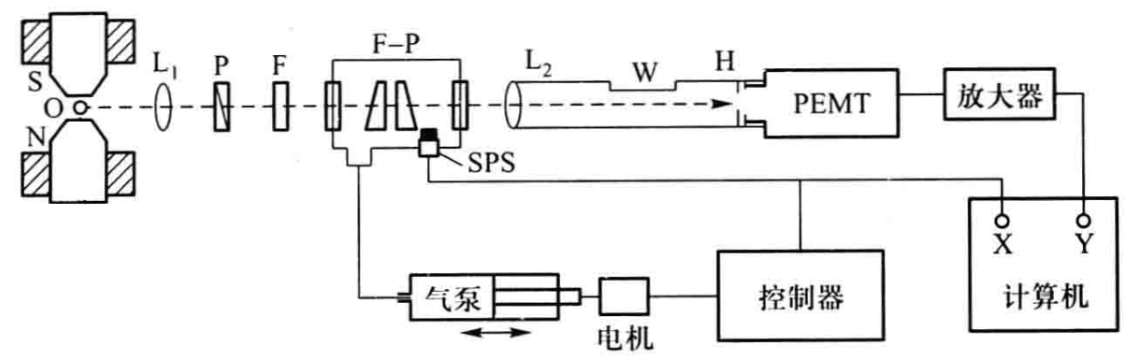
\includegraphics[width=0.85\linewidth]{fig/02.png}
    \caption{实验装置示意图.其中${\rm O}$为汞灯光源,${\rm N}$、${\rm S}$为电磁铁的磁极,${\rm L_1}$、${\rm L_2}$分别为准直透镜和成像透镜,F为透射干涉滤光片(投射峰值为${546.1\rm nm}$),${\rm SPS}$为半导体压力传感器,PEMT为光电倍增管,K为1/4波片.}
    \label{fig2}
\end{figure}
\autoref{fig2} 给出了沿垂直磁场方向观察塞曼效应的装置.实验装置主要分为扫描式F-P标准具和成像及监测系统.Hg发出的光通过透镜和滤光片之后进入F-P腔发生干涉,再通过${\rm L_2}$成像在针孔光阑上,光电倍增管(PEMT)PEMT可以检测等倾干涉环圆心处透过针孔光阑的光信号,其输出电信号经过放大器接入计算机的Y轴.半导体压力传感器(SPS)接入计算机的X轴,作为横向扫描信号,并通过气泵控制气室的压强.

利用 \autoref{fig2} 展示的装置,我们可以在计算机上控制测量光谱的过程,并且可以在计算机上直接看到光谱测量的结果.
\subsubsection{标准具的色散范围$\Delta \widetilde{\nu}_R$}
色散范围指光学器具所允许的不同波长的干涉花纹不重叠的最大波长差.对于F-P标准具来说,色散范围的定义为$$\Delta\lambda_R=\lambda_2-\lambda_1=\frac{\lambda^2}{2h},$$其中$h$为标准具间隔圈的间距.若被研究的谱线波长差大于仪器的色散范围时,两套花纹之间就会发生重叠或者错序,影响观察.

若用波数来表示,色散范围又可以写作$\Delta \widetilde{\nu}_R=1/2h$.例如标准具间隔圈的间距为$h$=2mm,\ $\Delta \widetilde{\nu}_R=1/2h=2.5\ {\rm cm^{-1}}$.说明标准具只能用来研究很窄的光谱范围.
\subsubsection{气压扫描系统}
由理论结果可以得到光线在二镜面间经过二次反射之后光程将增加$$\Delta l=2nh\cos \theta.$$本实验中使用的气压扫描式法布里-珀罗标准具可以通过改变腔内空气的密度(即改变气压)来改变折射率$n$,这样就可以连续改变光程差$\Delta l$,从而实现连续扫描干涉光谱序及序内光谱线.

气压扫描控制器扫描的时候,步进电机驱动封闭压缩泵用来改变气室内的气压,通过压力传感器直接输出与气压成线性关系的电压信号,作为X坐标信号输入计算机.从针孔后一次透过的子谱线光强信号经过光电接收器转换放大,作为Y坐标信号输入计算机,这样计算机就可以展现出塞曼分裂后各个子谱线的光强随气压(即随波数)的变化的曲线.
\subsection{实验过程}
\subsubsection{调节共轴光路}
点燃汞灯,检查汞灯是否位于磁场的几何位置中心.调节F-P标准具的位置,使得汞灯正好处于F-P标准具的中心轴线上.依次将准直透镜${\rm L_1}$和干涉滤光片F引入光路并调节共轴,使得正好能产生近似平行光入射到F-P标准具的窗口内.
\subsubsection{调节F-P标准具的准直度}
粗调F-P标准具的平行度:通过移动眼睛观察等倾干涉条纹中心的吞吐现象进行判断和调节.若眼睛向某个方向移动时在中心有亮斑``冒出来'',或中心圆环直径变大,则把这个方向的旋钮压紧或者把相反方向的旋钮放松(以减小这个方向的$h$).反复调节直到眼睛向各个方向移动时,观察不到吞吐现象.

细调F-P标准具的平行度:加磁场,并对F-P腔内气压进行连续扫描,根据眼睛从针孔光阑后观察等厚干涉图中心位置是否有移动进行判断.若看到有多条条纹向某个方向移动(升压时),则把这个方向的旋钮放松或者把相反方向的旋钮压紧(以增大这个方向的$h$).反复调节直到在压强变化时,中心位置没有移动为止.

调节结束后,取下针孔光阑,将光电倍增管套入H出射口并锁紧. 关闭控制器电源后,正确连接高压和信号线.连接光电倍增管旁侧的小灯电源,调节F-P俯仰倾斜,使得从观察窗口W可以看到汞等倾干涉环圆心和针孔光阑重合.随后关闭W窗口,打开高压电源.
\subsubsection{采集汞灯的塞曼分裂光谱}
打开计算机里的数据采集软件,设定合适的光电流量程将高压调整至-400 V附近.注意每次测量光谱之前都要进行放气操作,以使F-P腔内每次起始的气压都是一样的.在设置好参数之后,点击计算机软件中的``开始实验''即可进行自动测量.\cite{shouce}

在气压扫描控制器扫描时,依次测量:(1)无磁场作用时,汞灯546.1 nm的光谱图;(2)在1 T磁场(对应励磁电流为5.0 A)作用下,测量汞灯546.1 nm光分裂后的子谱线的光谱图;(3)在1 T磁场作用下,汞灯$\pi$线的光谱图;(4)在1 T磁场作用下,汞灯$\sigma$线的光谱图.
\subsubsection{复原器材}
扫描完成后,在计算机软件上点击``复位'',关闭汞灯,关闭控制器电源,取下光电倍增管,收拾桌面.


\section{实验结果与分析}
\subsection{塞曼谱线测量结果}
\autoref{fig3}展示了汞灯546.1 nm在无磁场,1 T磁场,和0.8 T磁场下的光谱图.从 \autoref{fig3}(a) 中可以知道,(在一个光谱周期内)光谱只有一个明显的峰,而周围的不太平整的凸起就是汞灯546.1nm线附近的精细结构和超精细结构.一般来讲,精细结构效应是比较弱的,一般的光栅分谱仪很难分辨,但是本实验使用的F-P标准具的分辨率足够高以使得我们可以比较轻松地分辨这些结构.加入磁场后,谱线发生分裂.从 \autoref{fig3}(b)和 \autoref{fig3}(c)中我们可以看出,(在一个光谱周期内)原来的546.1 nm线分裂成了9条子谱线,并且在1 T磁场下谱线的分裂比在0.8 T磁场下谱线的分裂更强.这说明磁场越强,谱线的分裂就越明显.

因为$\pi$光和$\sigma$光的偏振方向不同,所以通过在光路中加入滤波片,并改变其不同取向,可以只在光谱图上看到$\pi$和$\sigma$线. \autoref{fig5} 展示了在1 T磁场下,$\pi$线和$\sigma$线的光谱图.可以看到, \autoref{fig5}(a)中在一个周期保留的三条线是$\pi$线,而 \autoref{fig5}(b)中在一个周期保留的六条线是$\sigma$线,这和我们的预期也是相符的,因为通过 \autoref{eq5} 我们可以计算出,$\pi$线波长的偏离是要比$\sigma$线更大的.图中的一些没能滤去的峰可能是由于偏振片的滤光特性不是那么完美导致的.
\begin{figure}
  \centering
  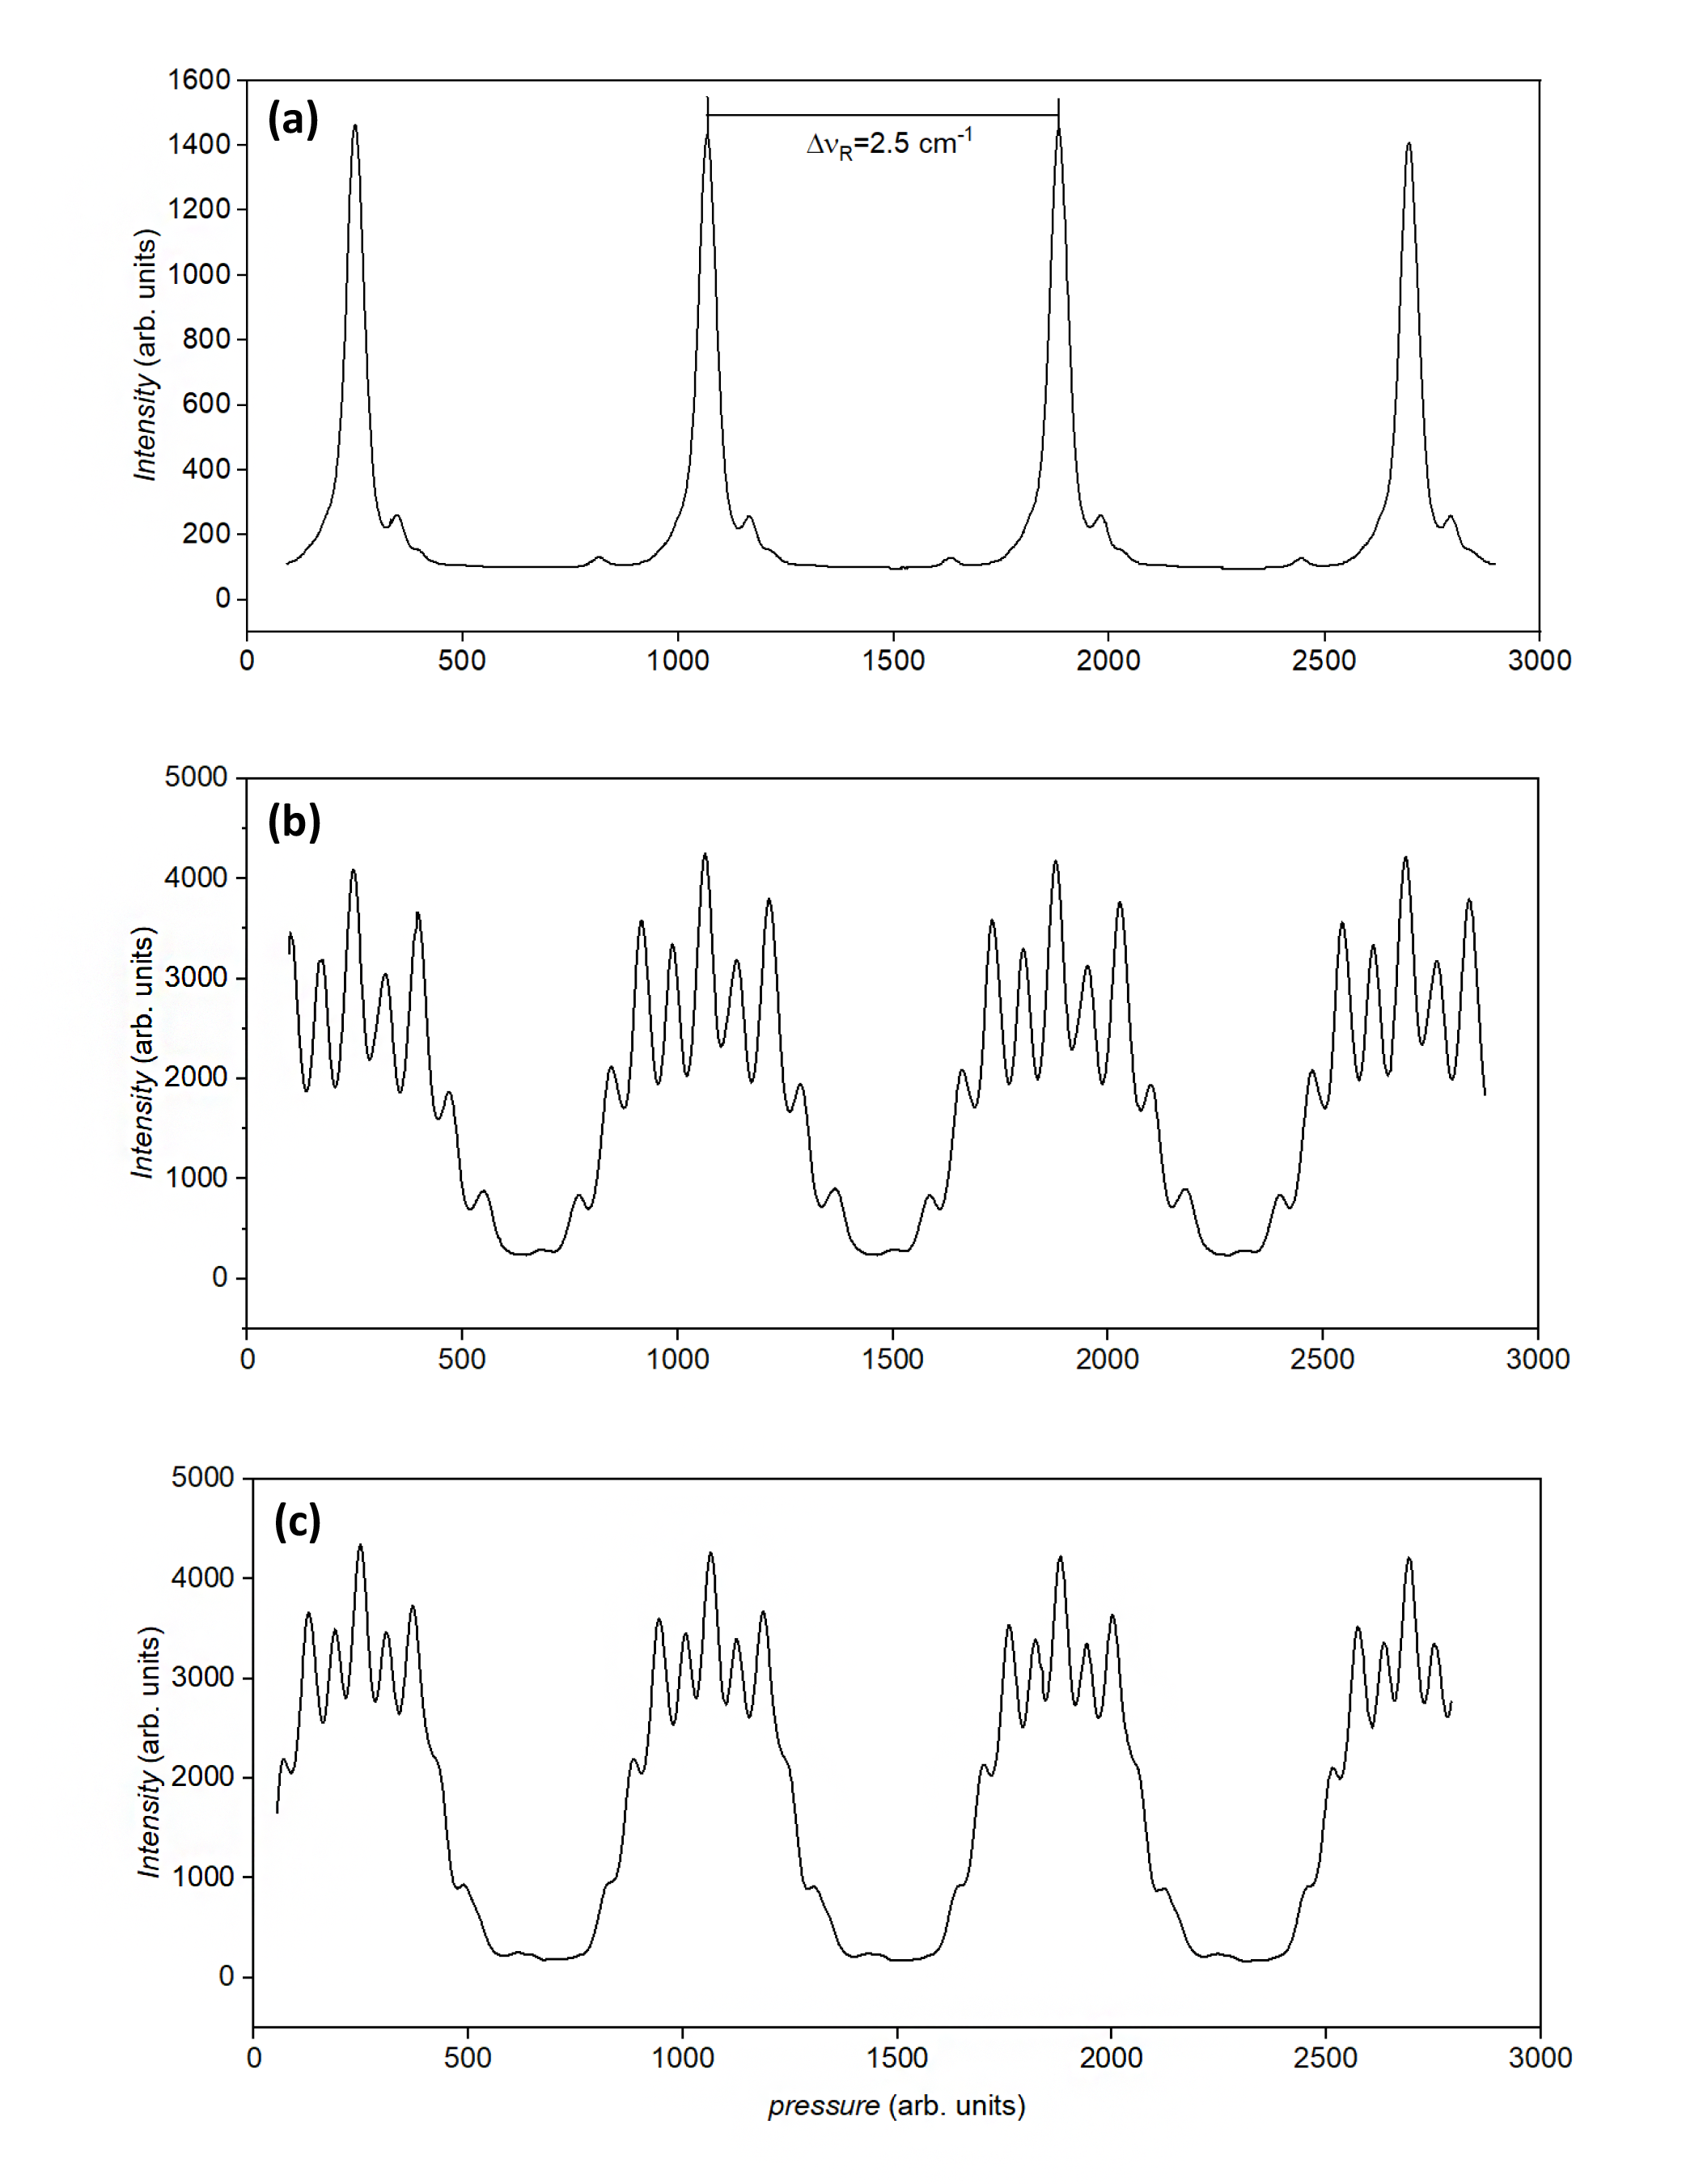
\includegraphics[width=0.95\linewidth]{fig/data1.png}
  \caption{汞灯光谱线的扫描结果1.横轴为气室的压强(任意单位),纵轴为光强(任意单位,注意由于实验过程中不同次测量时高压设置不同,不同图像间光强数字的相对大小是不同的).因为本实验使用的F-P标准具的自由光谱范围为$\Delta\widetilde{\nu}_R=2.5\ {\rm cm^{-1}}$,所以光谱的周期(波数差计)就应该是$2.5\ {\rm cm^{-1}}$.\ (a)无磁场作用时.\ (b)1 T磁场(激励电流为5.0 A)作用下时.\ (c)0.8 T磁场(激励电流为4.0 A)作用下时.}
  \label{fig3}
\end{figure}
\begin{figure}
  \centering
  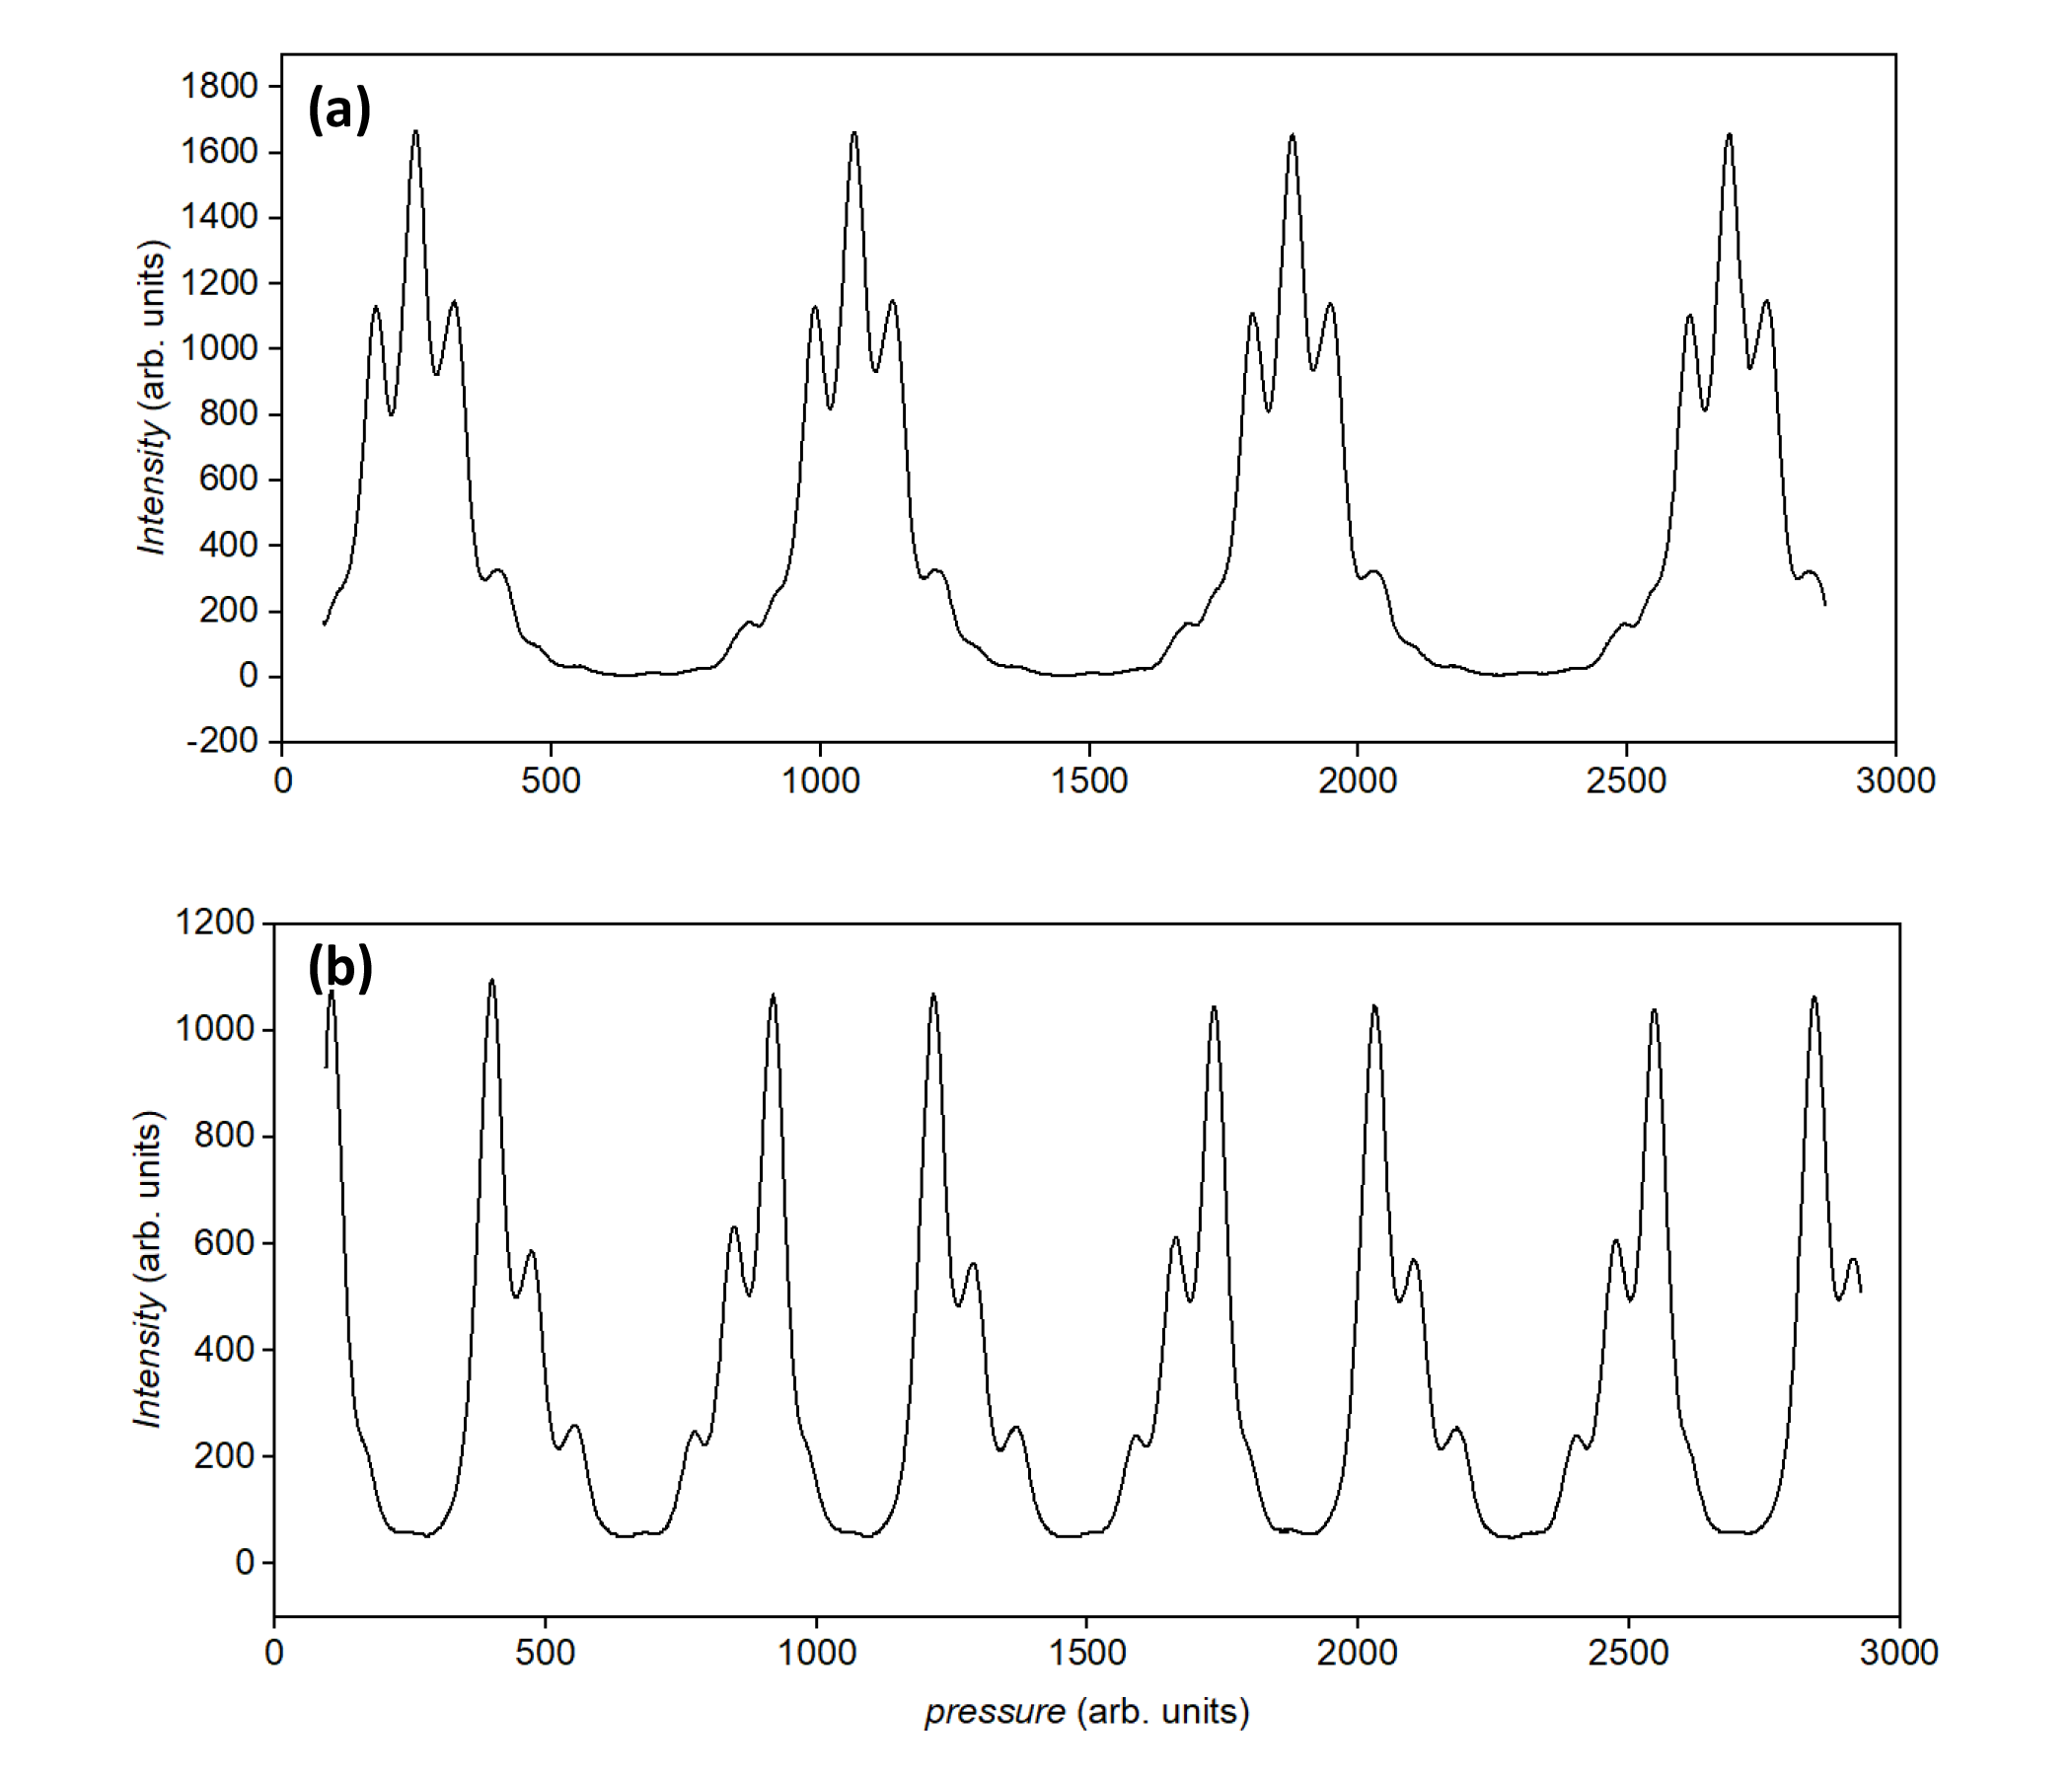
\includegraphics[width=0.9\linewidth]{fig/data2.png}
  \caption{汞灯光谱线的扫描结果2.\ (a)1 T磁场作用下,$\pi$线的光谱图.\ (b)1 T磁场作用下,$\sigma$线的光谱图.}
  \label{fig5}
\end{figure}
\subsection{各子谱线相对于546.1 nm谱线的波数差偏移}\label{deviation}

由于谱线之间间隔较近,产生了相互影响,所以我们实际观察到的子谱线并不是分立的,而是相互连在一起的.通过origin软件中的``Multiple Peak Fit''功能可以进行分峰拟合,找出不同峰值的位置. \autoref{fig4} 展示了origin软件在 \autoref{fig3}(b)的一个周期内($p\in[700,1500]$)做出的多峰拟合结果.通过拟合我们可以确定各个子谱线和546.1 nm线(峰值最高的谱线)的距离.

通过子谱线与主谱线的距离和光谱的周期的比值可以得到子谱线相对于主谱线的偏移. \autoref{tab1} 展示了子谱线偏移的测量结果以及与理论值的比较.

从 \autoref{tab1} 中我们可以看到,子谱线与546.1 nm谱线的波数差的实验值和理论值基本是吻合的,这是符合预期的.但是实验值和理论值还是产生了一定的偏离:每个实验值的绝对值都要比理论值的绝对值小,这可能有如下两个原因.

第一个原因是磁场强度的不准确.虽然操作手册上写着5.0 A的激励电流可以激发1 T的磁场,但是可能实际由于仪器的不准确,导致实际激发的磁场比1 T要小,这样根据 \autoref{eq6} 就可以知道实验中的洛伦兹单位比理论值要小,也就导致了子谱线与546.1 nm谱线的波数差的实验值比理论值要小了.

第二个原因是汞原子内部比较复杂的结构.546.1 nm谱线是双电子从${\rm 6s7s^3S_1}$跃迁至${\rm 6s6p^3P_2}$产生的,这和单电子跃迁的情形有一点区别,电子之间的耦合作用可能会导致这里的有效的荷质比和标准值有一定偏离.如果实验中电子的有效荷质比要小于标准值,那么同样的,根据 \autoref{eq6} 我们可以知道波数差的实验值要比理论值小.
\begin{figure}
  \centering
  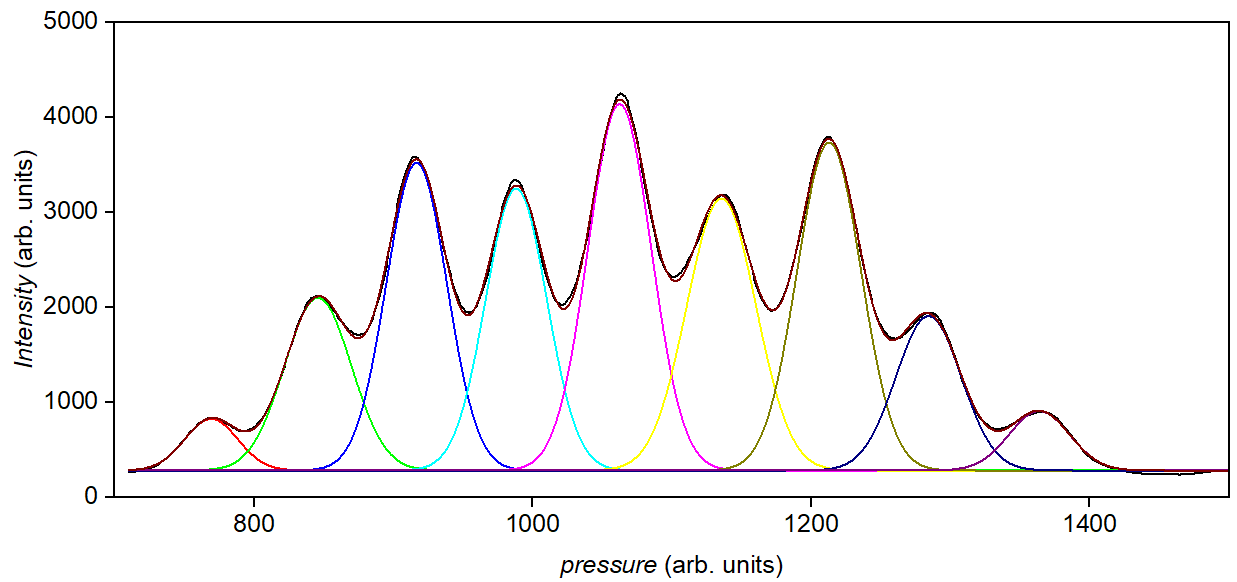
\includegraphics[width=0.78\linewidth]{fig/mul_peak_fit.png}
  \caption{汞灯光谱线一个周期内的多峰拟合结果(使用 \autoref{fig3}(b)的数据进行拟合,其中$p\in[700,1500]$).}
  \label{fig4}
\end{figure}

\begin{table}[h]
  \caption{外磁场为1 T情形下,各子谱线相对于546.1nm谱线的波数差偏移.波数差$\Delta\nu_{R}=2.5{\rm cm^{-1}}$对应的压强差$\Delta p=816.1$ (arb. units).}
  \label{tab1}
  \begin{ruledtabular}
    \begin{tabular}{cccccccccc}
      峰\footnote{这里我们546.1 nm的峰标记为0号峰,其余为磁场下分裂的子谱线,且向左向右分别标记为-1,-2,...和1,2,...号峰.} & -4 & -3 & -2  & -1 & 0 & 1  & 2  & 3  &4  \\ \hline
      $\overline{\Delta p}$ (arb. units)\footnote{这里的$\overline{\Delta p}$是由 \autoref{fig3}(b)中间的两个干涉序分别测量子谱线$\Delta p$后取平均值得到的,这样的操作能够减少非线性的影响.}& -293.1 & -216.6 & -145.8 & -74.2  & 0 & 73.2  & 150.4 & 221.8 & 301.3 \\ \hline
      $\Delta\nu_{R_{exp}}$ (${\rm cm^{-1}}$) & -0.898 & -0.663 & -0.447 & -0.227 & 0 & 0.224 & 0.461 & 0.680 & 0.923 \\ \hline
      $\Delta\nu_{R_{theo}}$ (${\rm cm^{-1}}$)\footnote{子谱线相对于546.1 nm谱线的波数差的理论值$\Delta\nu_{R_{theo}}$可由 \autoref{fig_spectrum} 得到,其中本实验使用的磁场强度$B$=1 T.} & -0.934 & -0.701 & -0.467 & -0.234 & 0 & 0.234 & 0.467 & 0.701 & 0.934 \\
    \end{tabular}
  \end{ruledtabular}
\end{table}

\subsection{各子谱线的相对强度}
通过origin软件中的``Multiple Peak Fit''我们不仅能够得到各个子谱线的位置,也能够得到子谱线的相对高度,即谱线的相对强度(去除基线值后). \autoref{tab2} 向我们展示了外磁场为1 T的情形下,各个子谱线的相对强度.其中谱线相对强度的理论值可以 \autoref{eq8} 得到.

通过对比,可以发现实验得到的子谱线相对强度和理论值基本上是可以一一对应的,但是实验值普遍来讲比理论值要更大,而且实验值明显有左右不对称的现象产生,这是在我们预期之外的.可能导致这个结果的有如下两个主要原因.

一是因为F-P标准具以及成像系统并不严格与磁场垂直.由 \autoref{eq8} 给出的相对光强是在垂直于磁场观察时才能得到的,但是在不垂直于磁场的地方,由于汞灯分裂谱线向四周发光不是各向同性的,于是在不同于垂直磁场的方向观察的时候可能就会发现光谱不对称的现象.

二是因为超精细结构的影响.如 \autoref{fig3}(a)所示,即使是在没有磁场的情形下,汞灯的光谱也不是完全对称的.在546.1 nm谱线峰的左右侧都有次峰,前面分析过这是超精细结构的影响,而在发生塞曼效应后,超精细结构也会对光谱产生影响,使得光谱和理想情况产生一定的偏移.

\begin{table}[]
  \caption{外磁场为1 T情形下,各子谱线的相对强度.其中5为546.1 nm的峰,其余为磁场下分裂的子谱线.}
  \label{tab2}
  \begin{ruledtabular}
  \begin{tabular}{cccccccccc}
  峰 & -4 & -3 & -2  & -1 & 0 & 1  & 2  & 3  &4 \\\hline
  Intensity (arb. units) & 541.9  & 1816.5 & 3236.2 & 2964.9 & 3854.6 & 2861.0 & 3450.6 & 1624.7 & 624.3  \\\hline
  相对546.1 nm线的强度         & 0.1406 & 0.4712 & 0.8396 & 0.7692 & 1      & 0.7422 & 0.8952 & 0.4215 & 0.1620 \\\hline
  相对强度\footnote{因为由 \autoref{eq8} 算出的$M_J=0\to M_J=0$谱线(即峰值最高的谱线)的相对光强为4,为了更好的将理论值和实验值相比较,这里我们将第5个峰的相对强度调整为4,其余子谱线的强度也等比例放大,这样对于整个光谱来说并没有本质的影响.}& 0.562  & 1.885  & 3.358  & 3.077  & 4      & 2.969  & 3.581  & 1.686  & 0.648  \\\hline
  相对强度理论值 & 0.5& 1.5&3 & 3&4  &3 &3  &1.5  &0.5       
  \end{tabular}
  \end{ruledtabular}
\end{table}
\subsection{根据光谱求荷质比}
若能求出洛伦兹单位$\widetilde{L}$,那么根据 \autoref{eq6} 我们就可以计算得到荷质比
\begin{equation}\label{eq_e/m}
  \frac{e}{m}=\frac{4\pi c\widetilde{L}}{B}.
\end{equation}
这里磁感应强度$B$=1 T且$c$为光速.

为得到洛伦兹单位,我们对 \autoref{tab1} 中的波数差做线性拟合.线性拟合的结果如 \autoref{fig6} 所示,由此我们得到洛伦兹单位(参考)$$\widetilde{L}=2k=0.452\ {\rm cm^{-1}},$$从而有荷质比$$\frac{e}{m}=1.70\times 10^{11}\ {\rm C/kg}.$$注意到这个值相比于标准值$(e/m)_{\rm std}=1.76\times 10^{11}\ {\rm C/kg}$来说要小一些(相对误差$\delta=3.41\%$),由于这里的计算完全和 \autoref{deviation} 是相反的(在 \autoref{deviation} 中我们是先假定了荷质比是标准值,然后通过磁场大小算出波数差的理论值,但是这里我们是利用波数差的实验值反推荷质比的有效值),所以这里产生误差的原因和 \autoref{deviation} 是一致的,这里不再赘述.
\begin{figure}
  \centering
  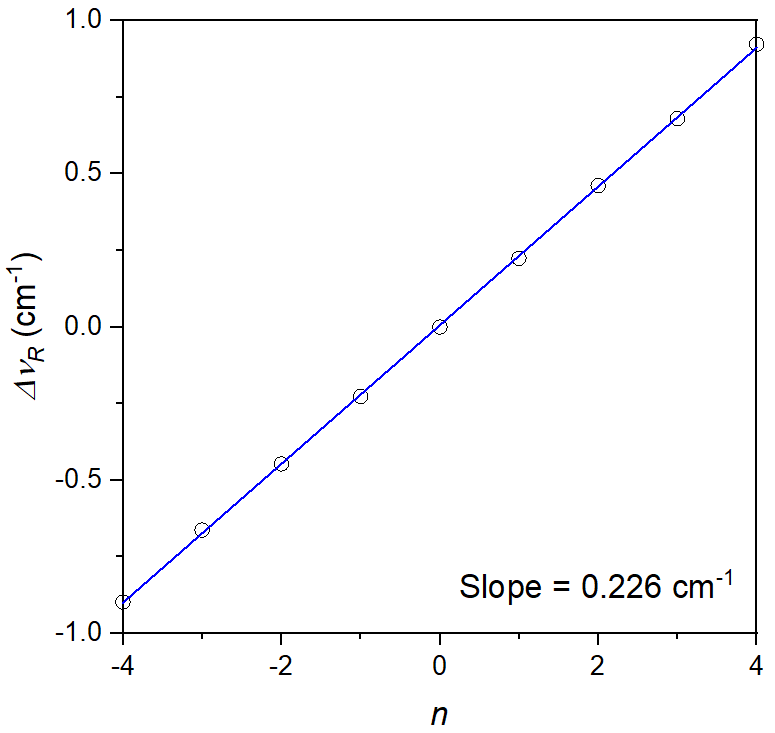
\includegraphics[width=0.45\linewidth]{fig/linear_fit.png}
  \caption{在外磁场为1 T的情形下,对波数差做线性拟合的结果,横轴为谱线峰的标号,纵轴为与546.1 nm线的波数差.拟合的斜率为$k=0.226\ {\rm cm^{-1}}$,相关系数$r=0.99993$.}
  \label{fig6}
\end{figure}
\section{结论}
本实验我们通过气压扫描式法布里-珀罗标准具对汞灯的546.1 nm谱线以及其在磁场下的塞曼光谱进行了观察.通过本实验的实验装置,我们可以实现在计算机上同时进行调节装置和记录光谱的操作,大大简化了实验流程,减小了误差.本报告给出了汞灯546.1 nm谱线在无磁场下,0.8 T磁场下,以及1 T磁场下的光谱图,还测量了1 T磁场作用下,$\pi$线和$\sigma$线的光谱图.之后,本报告对光谱图做了详尽的分析,计算了各个子谱线相对于546.1 nm谱线的波数差和相对强度,并与理论值进行了比较,发现和理论值基本一致,加深了我们对于塞曼效应的理解.最后,本报告通过塞曼光谱计算了电子荷质比.但是,由于时间有限,本报告并未能对光谱中与理论偏差的部分做出更加定量的解释.将来的实验还需更加深入研究汞灯546.1 nm谱线周围的现象,包括在更大范围的磁场下谱线的分裂情况,以及不同参数对谱线的影响.
\begin{acknowledgments}
  感谢刘开辉老师在实验过程中的操作示范和指导.感谢夏振灏、肖明暄同学协力完成了本实验.
\end{acknowledgments}

% bibliography 的参数是你的 *.bib 文件去掉后缀名后的部分

\begin{thebibliography}{}

  \bibitem{Book} 吴思诚, 荀坤. 近代物理实验(第四版). (北京: 高等教育出版社,2015).
  \bibitem{shouce} 汞原子546.1 nm谱线的塞曼效应观测仪器操作手册(实验室提供).
\end{thebibliography}
  
\clearpage % 附录前另起一页
\appendix % 附录开始
\section{思考题}
\subsection{从塞曼分裂谱中如何确定能级的$J$量子数?}
首先由于$\pi$线是磁量子数不变的跃迁放出的,所以通过数$\pi$线的数目就可以得到两个能级之间相等的磁量子数.如 \autoref{fig5} 所示,有3条$\pi$线,那么就可以知道两个能级之间有3个磁量子数是重合的,即-1、0、1.而$\sigma$线是磁量子数加1或者减1的跃迁,所以通过数$\sigma$线的数目就可以得到其中某个能级比另一个能级的磁量子数能取到的数多了多少.如 \autoref{fig5} 所示,有6$\sigma$线,说明其中一定有一个能级比另一个能级能够取到的磁量子数多2(即-2、-1、0、1、2).因此我们可以得到两个能级的$J$量子数一个是1一个是2,但是光凭借塞曼分裂谱我们不能知道这个光谱线是由$J=1$的能级跃迁到$J=2$的能级还是$J=2$的能级跃迁到$J=1$的能级,我们还需要知道能级之间的大小关系才可以确定(如 \autoref{fig_split} 所示).
\begin{figure}[h]
  \centering
  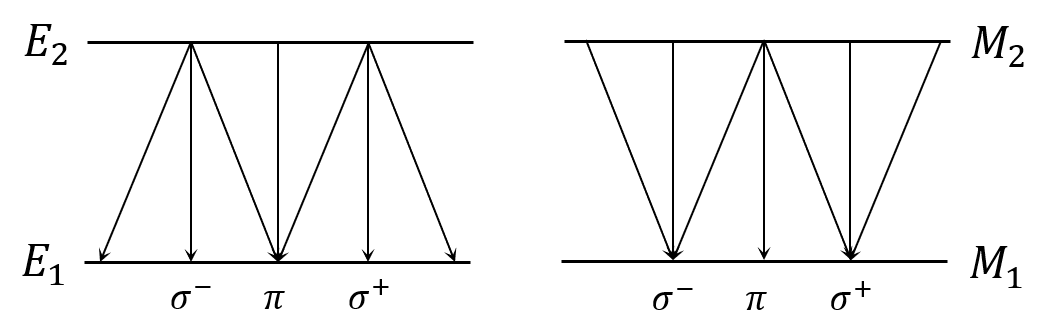
\includegraphics[width=0.8\linewidth]{fig/split.png}
  \caption{产生塞曼分裂谱的两种能级分布情况.左侧是由$J=1$的能级跃迁到$J=2$的能级,右侧是由$J=2$的能级跃迁到$J=1$的能级.}
  \label{fig_split}
\end{figure}
\subsection{根据塞曼分裂谱的裂距如何确定能级的$g$因子数?}
若已知本实验中546.1 nm线是由$J=2$的能级跃迁到$J=1$的能级放出的,那么根据 \autoref{eq5} 我们就可以知道各个子谱线的波数差(即裂距)和朗德因子$g_1$、$g_2$的关系(在这里我们应该认为洛伦兹单位$\widetilde{L}$是一个已知的量).由此我们就通过实验测量得到的波数差$\Delta\nu_R$算出两个两个能级的朗德因子.

\end{document}
